%\documentclass{acmsiggraph}                     % final
\documentclass[annualconference]{acmsiggraph}  % final (annual conference)
%\documentclass[review]{acmsiggraph}            % review
%\documentclass[widereview]{acmsiggraph}        % wide-spaced review
%\documentclass[preprint]{acmsiggraph}          % preprint

%% Uncomment one of the five lines above depending on where your paper is
%% in the conference process. ``review'' and ``widereview'' are for review
%% submission, ``preprint'' is for pre-publication, and ``final'' is for
%% the version to be printed. The ``final'' variant will accept the 
%% ``annualconference'' parameter, which changes the height of the space
%% left clear for the ACM copyright information.

%% The 'helvet' and 'times' packages define the typefaces used for
%% serif and sans serif type in this document. Computer Modern Roman 
%% is used for mathematics typesetting. The scale factor is set to .92
%% to bring the sans-serif type in line with the serif type.

\usepackage[scaled=.92]{helvet}
\usepackage{times}

%% The 'graphicx' package allows for the inclusion of EPS figures.

\usepackage{graphicx}

%% use this for zero \parindent and non-zero \parskip, intelligently.

\usepackage{parskip}

%% Optional: the 'caption' package provides a nicer-looking replacement
%% for the standard caption environment. With 'labelfont=bf,'textfont=it',
%% caption labels are bold and caption text is italic.

\usepackage[labelfont=bf,textfont=it]{caption}
\usepackage{subfigure}

%% If you are submitting a paper to the annual conference, please replace 
%% the value ``0'' below with the numeric value of your OnlineID. 
%% If you are not submitting this paper to the annual conference, 
%% you may safely leave it at ``0'' -- it will not be included in the output.

\onlineid{0}

%% Paper title.

\title{Advanced Medical Volume Rendering and Segmentation on the GPU}

\author{Mike Roberts \and Eric Penner \and Jeff Packer \and Mario Costa Sousa \and Joseph Ross Mitchell }
\affiliation{Hotchkiss Brain Institute, University of Calgary, Canada}

%%%%%% START OF THE PAPER %%%%%%

\begin{document}

\maketitle

\begin{figure}[t]
\centering
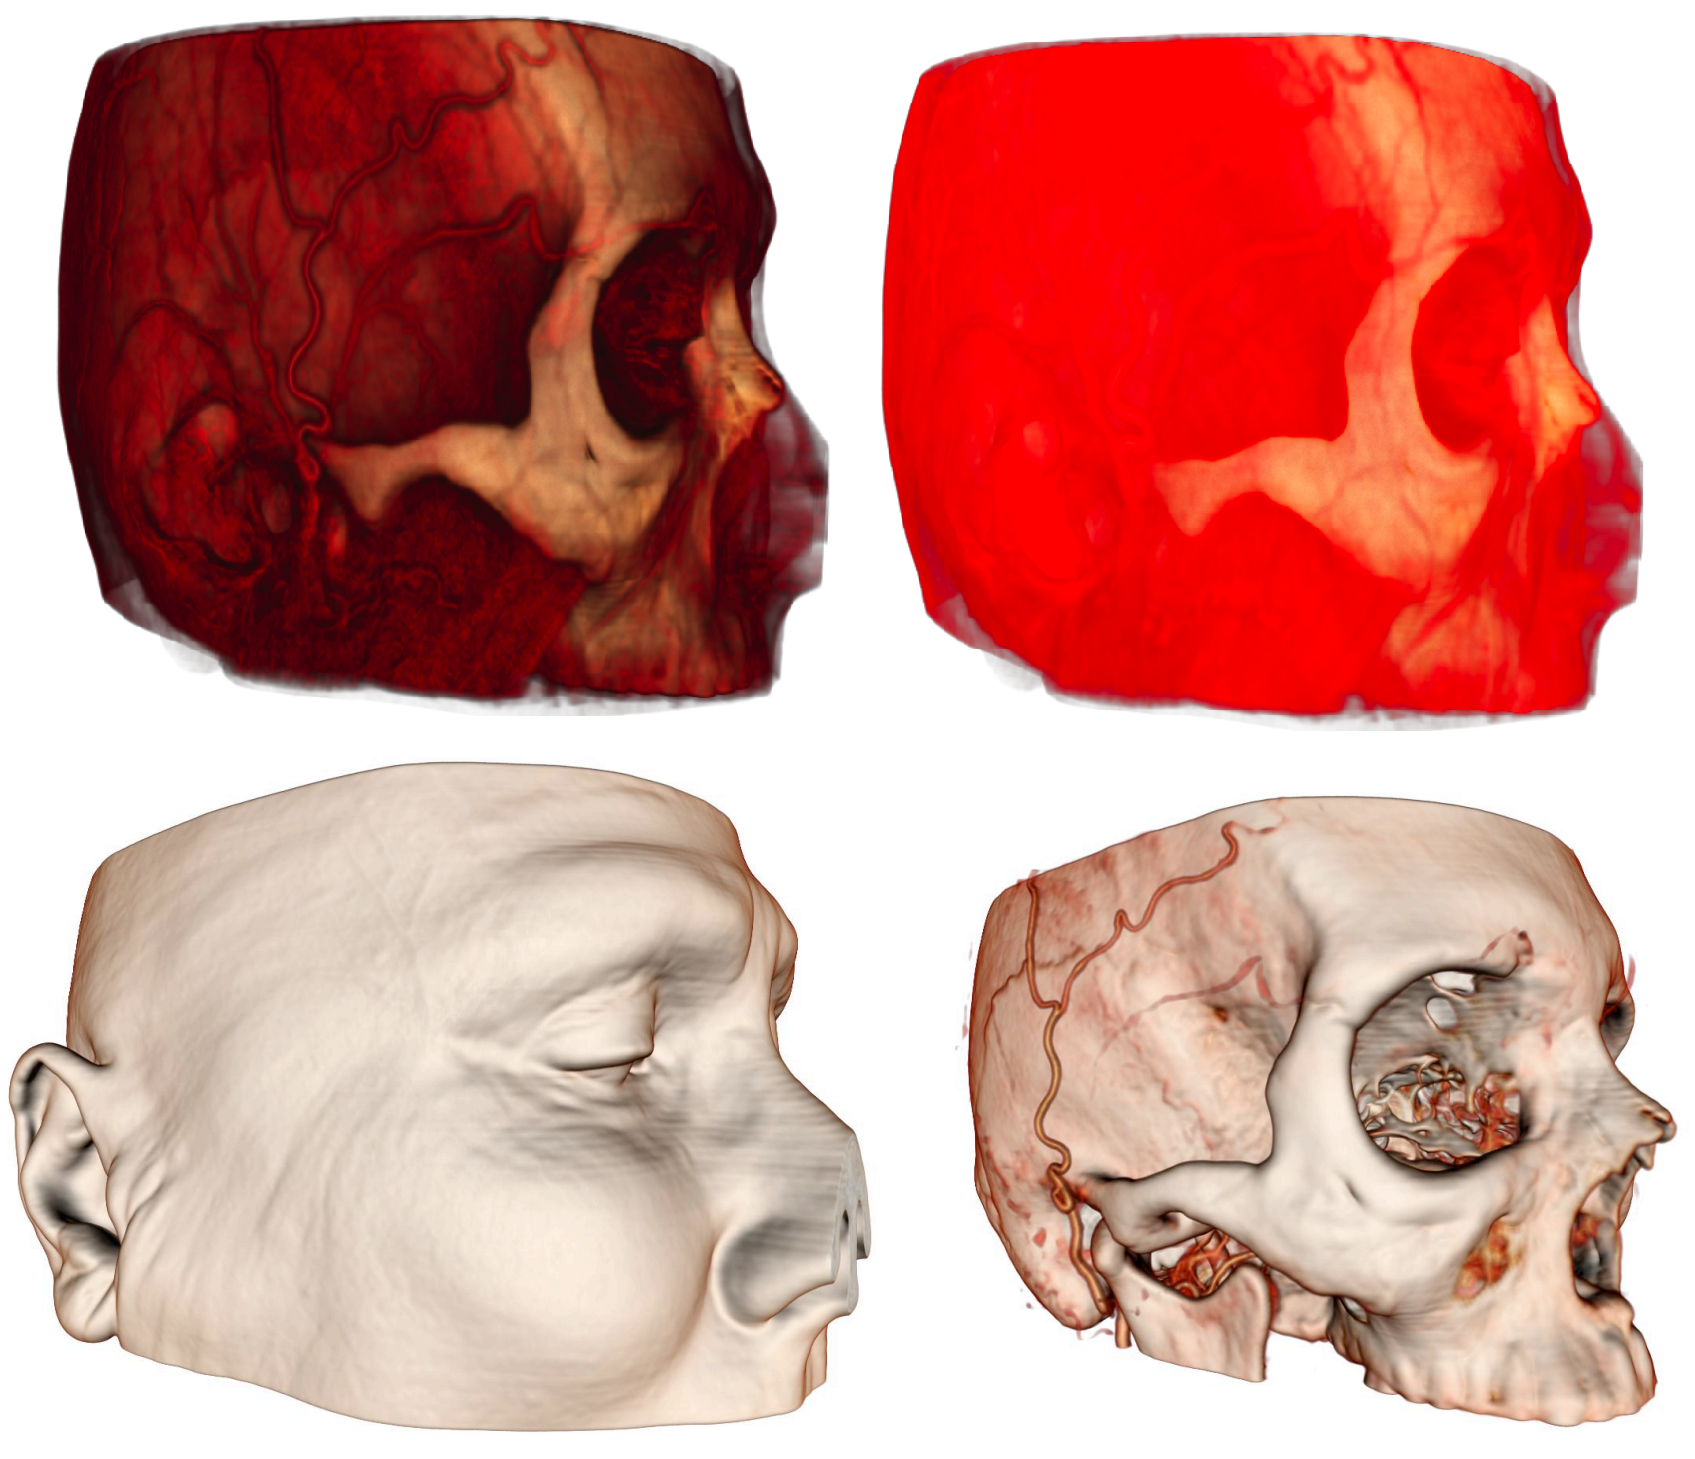
\includegraphics[width=3.3in]{figures/Eric-Composite.png}
  \caption{ Top Left: our GPU volumetric ambient occlusion algorithm visualizing a $512^3 $ CT data set at $30$ fps. Top Right: the same data set rendered with the same transfer function but without ambient occlusion. Ambient occlusion provides important perceptual cues about the structure and topology of the data set. In contrast to previous GPU algorithms, our algorithm supports interactive transfer function editing without requiring any costly preprocessing or  recomputation of auxiliary data structures. Bottom: our GPU hierarchical volumetric ray casting algorithm visualizing two different isosurfaces of the same data set at $130$ fps -- $15\times$ faster than unoptimized GPU volumetric ray casting with no reduction in rendering quality.}
\label{fig:visualization}
\end{figure}


\begin{figure}[t]
\centering
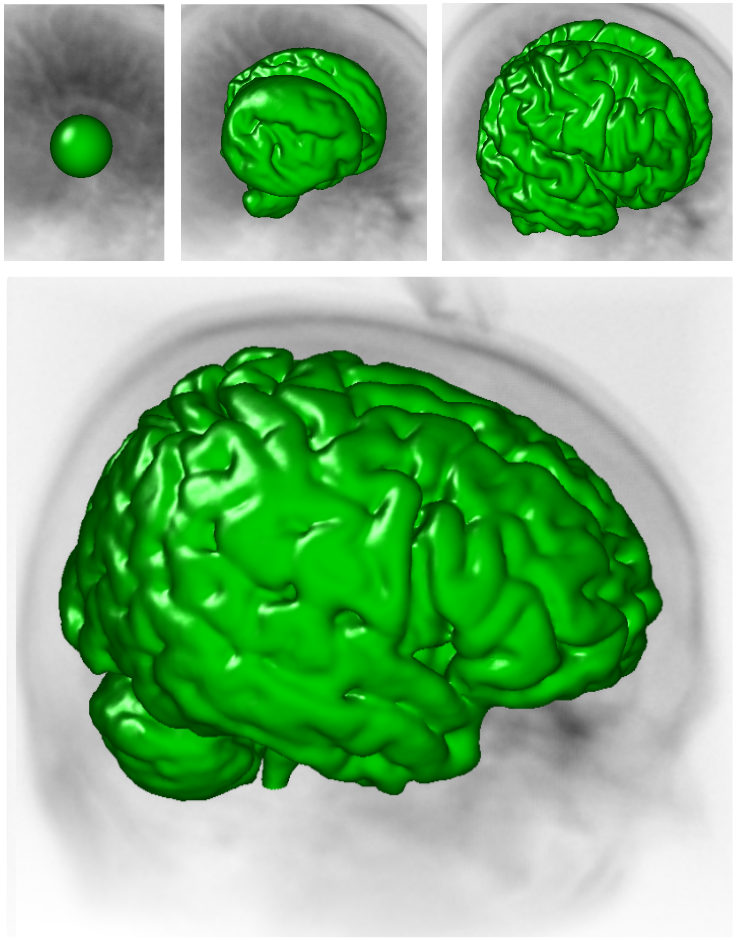
\includegraphics[width=2.9in]{figures/Brainweb-3D-Composite-Offset.png}
  \caption{ Our GPU level set segmentation algorithm interactively segmenting the brain matter in a noisy (signal-to-noise ratio of $11$) $256^3$ MRI in $7$ seconds -- $14 \times$ faster than previous GPU algorithms with no reduction in accuracy. }
\label{fig:segmentation}
\end{figure}

Volumetric visualization plays an important role in many image-guided surgical procedures, and is an important investigative tool in diagnostic medicine. Identifying the distinct regions in volumetric images -- a task known as \textit{segmentation} -- is also an important diagnostic tool.

As a physician interactively explores and takes measurements of a volumetric medical data set, the tasks of visualization and segmentation complement each other: an initial visualization can help a physician to roughly identify regions of interest within the data set; interactive segmentation methods can precisely quantify those regions with minimal user interaction; and those segmented regions can inform the interactive visualization and subsequent exploration.

We present three novel GPU algorithms that improve the quality and interactivity of the work-flow described above:

\begin{enumerate}
\item 
A volumetric ambient occlusion algorithm that improves image quality by providing important perceptual cues about the structure and topology of the data set (Figure~\ref{fig:visualization}). In contrast to previous algorithms~\cite{Ropinski-2008}, our algorithm supports interactive transfer function editing without requiring any costly preprocessing or recompututation of auxiliary data structures.
\item 
A hierarchical volumetric ray casting algorithm that is $15\times$ faster than unoptimized volume ray casting without affecting image quality (Figure~\ref{fig:visualization}).
\item 
A work-efficient level set segmentation algorithm that is $14\times$ faster than previous algorithms~\cite{Lefohn-2004} and improves the asymptotic step-completexy of previous algorithms~\cite{Jeong-2009,Lefohn-2004} without affecting segmentation accuracy.
\end{itemize}

For a more comprehensive description of these algorithms we refer the reader to our recent work~\cite{Roberts-2010,Penner-2009,Penner-2008}.

\tiny{
\bibliographystyle{acmsiggraph}
\nocite{*}
\bibliography{template}
\end{document}
}
